\documentclass[a4paper]{article}
\usepackage[margin=1in]{geometry}

\usepackage[english]{babel}
\usepackage[utf8]{inputenc}
\usepackage{amsmath}
\usepackage{amsfonts}
\usepackage{natbib}
\usepackage{graphicx}
\usepackage[auth-sc,affil-sl]{authblk}
\usepackage[colorinlistoftodos]{todonotes}
\usepackage{hyperref}
\usepackage{enumitem}
\usepackage{xcolor,colortbl}
\usepackage{array}

\renewcommand{\arraystretch}{2}

\title{User Interface Evaluation of the CP's Website\\ (Proposal)}
\author[1]{Luís  Cruz}
\affil[1]{MAP-i\\ Joint Doctoral Programme in Computer Science}
\date{January 4, 2014}

\begin{document}
\maketitle

\begin{abstract}
  This document proposes an usability evaluation for the website of the company \emph{CP -- Comboios de Portugal}. The company and the website are briefly described, as well as the users focused by the evaluation and the supported tasks. One analytical method and one empirical method are going to be applied in this evaluation: \emph{Heuristic Evaluation} and the \emph{Usability Test}, respectively, both described in this document.
\end{abstract}

\section{Introduction}

This project aims to evaluate the user interface of CP.pt\footnote{Available at: \url{http://www.cp.pt}} --- the official website of \emph{CP - Comboios de Portugal, E.P.E}.

CP is a public portuguese company responsible for rendering national and international passenger rail services. In the year 2012, CP had 4690 employees, transported 122 million passengers and almost 8713 thousand metric tons~\citep{CP2012aa}. They provide 3 main kinds of rail transportation services: \emph{urban} in the cities of Oporto and Lisbon; \emph{National} with regional services and the fast lines of \emph{Alfa Pendular} and \emph{Intercidades}; and \emph{International}.

Through the website, CP's customers can check the timetables, buy tickets, get information about the available lines and special offers and read some news related with CP services. In order to buy tickets, the website provides the \emph{netTicket} service, which requires the customers to have an account in their \emph{myCP} service and it is only available for the long distance trains \emph{Intercidades} and \emph{Alfa Pendular}.

According to the website the graphical interface was optimally designed for windows with $800\times 600$ pixels of resolution. A view of the website is depicted in the figure~\ref{fig:cp_home}, using a window with the same resolution. 

\begin{figure}[h] 
	\centering
	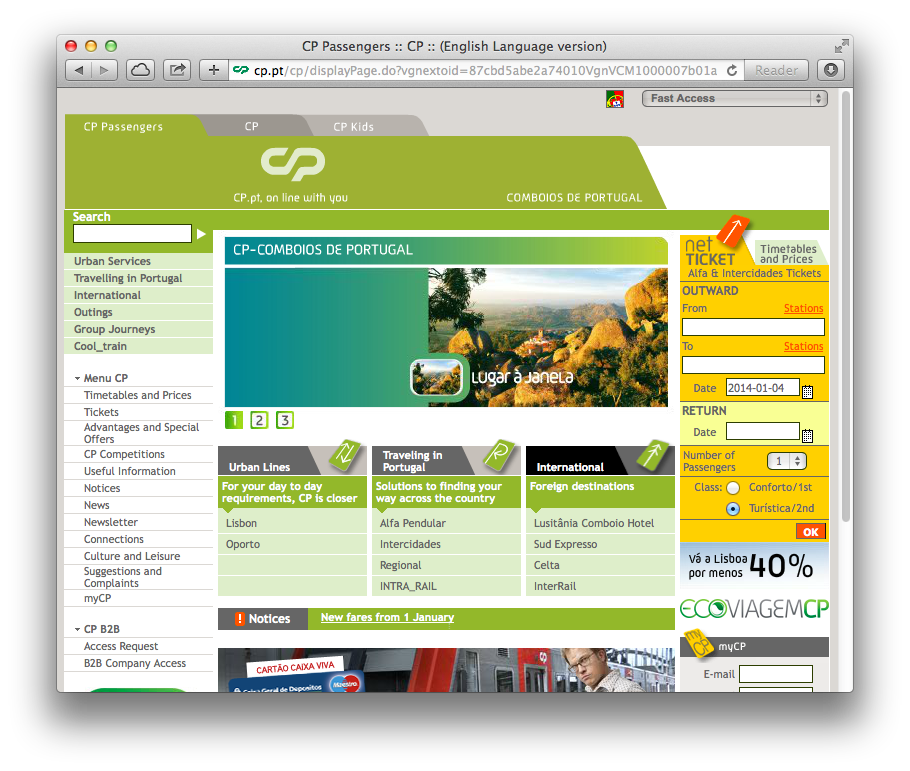
\includegraphics[width=\textwidth]{figures/cp_home}
 	\caption{View of the main page of CP.pt website in a window with resolution $800\times 600$ pixels, using the internet browser Safari Version 7.0.1.}\label{fig:cp_home}
\end{figure}

\section{Users and Context}
\label{sec:users_context}

CP customers vary according to the service provided. Many college students, workers and pensioners use the regional and urban services for small and medium distances. Long distance services are more used by college students that are away from home, tourists, and executive workers. Unfortunately, no official document stating the segmentation of the CP.pt website's users was found.

It is noticeable that CP services have a lot more passengers during school time, which means that students are an important segment of CP's customers. Besides, most of the students have good experience with the WEB, so the CP.pt website is expected to be a great tool to them. Therefore, this usability evaluation will focus in the segment of college students, which might be portuguese citizens as well as foreigners that study or want to study in Portugal and are able to speak English.

Many scenarios can apply for the use of the website by students. Some times they leave the classes earlier and need a way of quickly check if there are other alternative trains that can take them home earlier. Also sometimes there is no direct train to their destination, so they have to catch another in the the middle of the travelling. Another scenario is when the weekend is over and the student has to buy his/her ticket from home to his/her university city. Buying it from the website is more convenient since the student can avoid wasting time in the ticket lines and can grant a seat for his/her trip. Therefore, the following two contexts are considered the most important in terms of usability:

\begin{itemize}
  \item Check the timetable to find any suitable train for the trip and the respective prices.
  \item Buy a ticket for long distance trains with reserved seats.
\end{itemize}

\section{Usability Evaluation Methodology}

The evaluation will be taken using two paradigms: \emph{Analytical} and \emph{Empirical}.

\emph{Analytical} methods do not need to involve users --- they are based on inspection methods. Some well known analytical methods are the \emph{Heuristic Evaluation} (HE) proposed by \citet{nielsen1990heuristic}, the \emph{Cognitive Walkthrough} \citep{wharton1994cognitive} and its variant \emph{Streamlined Cognitive Walkthrough} \citep{spencer2000streamlined}.

\emph{Empirical} methods involve the user in the evaluation process through Usability tests, involving \emph{observation} and \emph{query} techniques, through \emph{controlled experiments}, in a more scientific approach, or even \emph{questionnaires}, \emph{focus groups}, etc. 

In this evaluation, the used analytical method will be the  \emph{Heuristical Evaluation} and the empirical method will be the \emph{Usability Test}. These methods are described in the next sections.



%----------------------------------------------------------------------------------------
%	Heuristic Evaluation
%----------------------------------------------------------------------------------------
\section{Heuristic Evaluation}

The elected analytical method for this evaluation was the \emph{Heuristic Evaluation}, because it is cheap, intuitive, easy to motivate people to do it and provides that useful results can be obtained~\citep{nielsen1990heuristic}.

\subsection{Methodology}
This method proceeds by having a small set of evaluators judging the system according to some general principles of interaction design, \emph{usability heuristics}. It has been shown that a number of evaluators between 3 and 5 provides good results and that there is no point in having more than 10 evaluators \citep{nielsen1990heuristic}. \citet{nielsen1995ten} proposed the 10 most important usability heuristics for User Interface Design:

\begin{itemize}
	\item Visibility of system status

	\item Match between system and the real world

	\item User control and freedom

	\item Consistency and standards

	\item Error prevention

	\item Recognition rather than recall

	\item Flexibility and efficiency of use

	\item Aesthetic and minimalist design

	\item Help users recognise, diagnose, and recover from errors

	\item Help and documentation.
\end{itemize}

Heuristic evaluation was originally developed for evaluators who had some knowledge in usability but who were not necessarily usability experts~\citep{nielsen1990heuristic}, however, it has been showed that the method is also very effective for expert evaluators~\citep{nielsen1992finding}.

In order to group the findings of this heuristic evaluation, the severity ranking proposed by \citet{nielsen1995rating} with a scale from 0 to 4:

\begin{enumerate}[start=0, label={\theenumi{} -}]
\item I don't agree that this is a usability problem at all;
\item Cosmetic problem only: need not be fixed unless extra time is available on project;
\item Minor usability problem: fixing this should be given low priority;
\item Major usability problem: important to fix, so should be given high priority;
\item Usability catastrophe: imperative to fix this before product can be released.
\end{enumerate}

In this evaluation, two experienced evaluators participated.

\subsection{Results}

After completing the heuristic evaluation \todo{number of problems} XX problems were found. They were sorted in the table according to the 
\begin{table}[h]
\begin{center}
  \footnotesize
\begin{tabular}{c | p{8cm} | c | p{4.5cm}}
  \hline
	\# & Problem & \parbox[c]{1cm}{Severity Rating} & Violated Heuristic  \\
	\hline
	
		1  &  The ``Timetable and Prices" form is very similar with the form for buying tickets. Non expert users might not notice the difference.    & \cellcolor{red!25} 3 & Error prevention  \\
		
		2 &  There is an auto complete feature in the "Timetable and Prices" and NetTicket forms, which whenever the user misspells a letter of the station name, the system may complete with another station's name, and the user has to hit the backspace button one more time than usual. & \cellcolor{red!25} 3 & Error prevention; Help users recognize, diagnose, and recover from errors.\\
	
  3   & The seat selection is made in a uncommon way. One has to first click on the previous seat and then on the desired seat.  & \cellcolor{red!25} 3 &  Consistency and standards  \\
  
		4  & The services of trains are defined as acronyms which are not used by the users (eg., IC means Intercidades)  &\cellcolor{orange!20} 2  &  Consistency and standards; Match between system and the real world.  \\
	

	5  &  When an unregistered user wants to buy a ticket after choosing a specific train, the system asks him/her to register but after finishing the registration, he/she has to search again for the same train.    & \cellcolor{orange!20} 2 &  Recognition rather than recall. \\

6 &  In order to check the price in the timetable it is necessary to click in a link which when clicked replaces itself into the respective price, but only for one train at a time. & \cellcolor{orange!20} 2 & Flexibility and efficiency of use.\\


7 &  When searching for a travelling ticket to buy, the user selects whether is travelling in first or second class in the beginning of the search. It is defined as second class by default and might not be perceptible. Through the next steps the user cannot change it. & \cellcolor{orange!20} 2 & User control and freedom.\\

8 & In the buying process there is no back button, besides the one provided by the browser that is not recommended by the system since he presents an alert warning that the user is about to leave the page. & \cellcolor{orange!20}2 & User control and freedom\\

9  &  In the timetable results, there is a clickable down arrow that does not do anything  & \cellcolor{yellow!10} 1 &  Aesthetic and minimalist design, Consistency and standards  \\

	10  &  There is a Time input field when in the form "Timetables and Prices", which might be unnecessary and provides no useful filtering in the results.  & \cellcolor{yellow!10} 1 &  Aesthetic and minimalist design  \\
	
		11 &  In the timetable results there is a number identifying the row that does not provide any useful information & \cellcolor{yellow!10} 1 & Aesthetic and minimalist design\\
	
\hline
\end{tabular}
\end{center}
\caption{default}
\label{heuristic evaluation details}
\end{table}

\paragraph{Evaluator 1} Sth

\paragraph{Evaluator 2} Sth la la la la llaa

%----------------------------------------------------------------------------------------
%	USABILITY TEST
%----------------------------------------------------------------------------------------
\section{Usability Test}

% ---------- PARTICIPANTS --------- %
\subsection{Participants}
A careful selection of participants --- it is important to have participants with the same experience level, demographics, and areas of interest, and that will eventually be the end users of the product --- the Screener method is very useful in this phase~\citep{mitchell2007step};
% ---------------~o~--------------- %


% ------------- TASKS ------------- %
\section{Tasks}


The tasks that the participant has to accomplish are the following:

\begin{enumerate}
  \item Select the English Version of the application.
  \item Find the schedule for a trip from Braga to Aveiro.
  \item Find a cheap trip from Braga to Aveiro.
  \item Buy a ticket from Braga to Porto.
\end{enumerate}

These tasks are described in more detail in the \emph{Usability Test Plan}, available in the appendix~\ref{sec:usabilityTestPlan}.
% ---------------~o~--------------- %


% - Moderator's Guide and Data Logging - %
\subsection{Experimental Design}

In order to guide the moderator during the experiment, a script was elaborated providing the moderator with a clear description of the all steps that that are necessary to efficiently accomplish all the tasks.

\todo{independent and dependent variables and usability measures to be used.}

As suggested in~\citep{mitchell2007step} it is beneficial for the moderator to get the participant's opinion during the test session.
The usability test combined both \emph{observation} and \textit{query}.

 The participant will be asked to think aloud, describing every step he/she makes during the tasks. The moderator will be directly observing the participant and taking some notes using the Data Logging Form, provided in appendix~\ref{sec:dataLoggingForm}, and after each task the moderator makes a short interview focusing in the questions provided in the Usability Test Plan (see appendix~\ref{sec:usabilityTestPlan}). The screen and the audio is also recorded for indirect observation.

 After the completion of each task the participants answer a short questionnaire, as well as after the whole test they answer a post-test questionnaire. Also, they are interviewed by the moderator in an informal way, trying to answer some questions clearly stated in the Usability Test Plan document (see ~\ref{sec:usabilityTestPlan}). 
% ---------------~o~--------------- %



% ----------- Workplace ----------- %
\subsection{Workplace}
It is important to create a workplace regarding features that might affect the results.

According to \citep{http://www.satya-weblog.com/2013/07/desktop-laptop-mobile-screen-resolution-most-common-worldwide.html}, the most common resolution used in WEB is $1366\times 768$, so in this experiment a screen with approximately the same resolution is used: $1440\times 990$.

For accessing the application, the browser Safari 7.0.1 with default settings is used. The internet connection has an average download and upload speeds of $4 Mbit/s$ and $1Mbit/s$, respectively. The screen and audio is recorded using the tool QuickTime Player 10.3. During the test, the moderator stands next to the participant which has free access to the laptop, taking in account that the participant feels comfortable.
% ---------------~o~--------------- %



% ------------ RESULTS ------------ %
\section{Results}
The reports of the usability test comply with the Common Industry Format (CIF) supporting a summative usability evaluation \citep{iusr2006cif}.
% ---------------~o~--------------- %

\appendix
\section{Consent and Recording Release Form}
\todo{reference}

I agree to participate in the study conducted and recorded by the MAP-i student Luís Cruz. 

I understand and consent to the use and release of the recording by Luís Cruz. I understand that the information and recording is for research purposes only and that my name and image will not be used for any other purpose. I relinquish any rights to the recording and understand the recording may be copied and used by Luís Cruz without further permission. 

I understand that participation in this usability study is voluntary and I agree to immediately raise any concerns or areas of discomfort during the session with the study administrator.

Please sign below to indicate that you have read and you understand the information on this form and that any questions you might have about the session have been answered. 

Date: \rule{2cm}{0.4pt} 

Please print your name: \hrulefill

Please sign your name: \hrulefill


Thank you!

Your participation is kindly appreciated.


\section{Usability Test Plan}
\label{sec:usabilityTestPlan}
This document is a script for the moderator describing the sequence of activities and questions that each participant will experience.

\subsection{Introductory Talk}

The moderator introduces himself and explains to the participant what is his role and how the experiment will evolve.

It is important to make the participant feel comfortable to give his honest opinion and do not worry to say something that could hurt the developer's feelings. We want to listen to every comment the user might have about the website, and the ``Thinking Aloud" technique should be explained to him for better results.

It is recommended before starting to ask if the user has any doubts about the consent form he just signed as well as about the experiment.
 
\subsection{Tasks}

The computer is set with an open browser to: \url{http://www.cp.pt/}

In this section the tasks are detailed with all the necessary steps in order to help the moderator to help the user. However, unless the user needs some help he/she is not supposed to read it.

After each task, the moderator reports if the user accomplished the task with the following taxonomy: \emph{Yes} / \emph{No} / \emph{Yes with help}.

\paragraph{Task 1 - Select the English Version} In this task the user has to change the language of the application to English:

\begin{enumerate}[label=\roman*.]
  \item Go to the CP.pt homepage (url: \url{http://www.cp.pt/}) 
  \item Select the british flag on the top bar.
\end{enumerate}
\subparagraph{Completion Criteria:} The website has to be in the English language.

\subparagraph{Post-task Interview:}

\begin{enumerate}[label=1.\theenumi .]
  \item Is this the first time you visit this website?
  \item Please give me your first impressions about the layout and design of the website.
  \item How easy or difficult was it for you to accomplish this task?
  \item Was there something specific that made this task easy or difficult?
\end{enumerate}

\paragraph{Task 2 - Going from Braga to Aveiro} In this task the user is asked to find when is the next train from Braga to Aveiro, how much is the ticket and where is it necessary to switch lines. In order to accomplish this task, the user has to:

\begin{enumerate}[label=\roman*.]
  \item Go to the CP.pt homepage
  \item Find the form through the tab ``Timetables and Prices" of the right panel.
  \item Introduce the details of the trip, from Braga to Aveiro in the present day. Optionally, the time can be set, and it is not necessary to specify the return trip.
  \item Select one of the listed trips, by selecting ``see" and/or ``detail" links. 
  \item Report the time of departure, the price of the ticket, the duration and how long will the passenger have to wait in the station, and when is the departure of the second train.
\end{enumerate}

\subparagraph{Completion Criteria:} The user is able to say when is the departure, when the train arrives to the destination and where is the train scale.

\subparagraph{Post-task Interview:}

\begin{enumerate}[label=2.\theenumi .]
  \item How easy or difficult was it for you to accomplish this task?
  \item Was it easy to find the form?
  \item Did you like the way you had to input the trip details?
  \item Did you clearly understand the results table?
  \item Which part of the task you found more confusing?
  \item When you clicked in the details of your trip, did you find it easy to check when you have to switch trains?
   \item Do you feel that you need to ask some extra information to the ticket officer?
\end{enumerate}


\paragraph{Task 3 - Find a cheap ticket from Braga to Aveiro}
This task is similar to the previous task 2 but this time, the passenger only has 10 euros to spend in the trip. The steps are the same, but in this case the user cannot select a fast train IC or AP, because they are more expensive.

\subparagraph{Post-task Interview:}

\begin{enumerate}[label=3.\theenumi .]
  \item How easy or difficult was it for you to accomplish this task?
  \item Which part of the task you found more confusing?
  \item When you clicked in the details of your trip, did you find it easy to check when you have to switch trains.
  \item What is your opinion of how price information is displayed?
\end{enumerate}

\subparagraph{Completion Criteria:} The user chose a train from Inter-regional or Urban services and he/she is able to say when is the departure, when the train arrives to the destination, and how much is it going to cost.


\paragraph{Task 4 - Buy a ticket from Braga to Porto}
In this task the user will be using the netTicket feature to buy a ticket for the train \emph{intercidades} (IC) from Braga to Porto. This will include the registration in myCP service and the task ends before the payment step in order to simplify the test setup. This task intends to analyse how an unregistered user manages to buy a ticket. This might be a difficult task.

The steps are the following:

\begin{enumerate}[label=\roman*.]
  \item Go to the CP.pt homepage.
  \item Find the form netTicket in the right panel.
  \item Insert in the \emph{from} field, the value \emph{Braga}, and in the field \emph{To} the value \emph{Porto - Campanhã}. Specify the dates for the trip, including return.
  \item Choose the two trains for the round trip and click ``continue" to proceed to the next step.
  \item Since the user is not registered yet, the user clicks on the link ``Register"
  \item The user fills the registration form submits.
  \item A new form asking for Preferred/Most used Service appears. It is optional, the user can skip it.
  \item A new form asking if CP can use the email for newsletter. The user can now finish the registration.
  \item The user has to resubmit the trip information.
  \item Now the user identifies the passenger with his/her name and ID Card number
  \item Select one seat different from the default when available. In the end click ``Confirm"
\end{enumerate}

\subparagraph{Completion Criteria:} The user is on stage 5 ``Payment" of the buying process. In the description of the page, the details of a trip from \textit{Braga} to \textit{Porto - Campanhã} are summarized.

\subparagraph{Post-task Questions:}

\begin{enumerate}[label=4.\theenumi{}.]
  \item How easy or difficult was it for you to accomplish this task?
  \item Which part of the task you found more confusing?
  \item What did you think about the registration process?
  \item When you had to select the seat for your ticket, the interface was familiar? Did you have any trouble understanding how it works?
  \item What is your about opinion how the price information is displayed?
  \item In the whole task was there any steps that you found unnecessary? Which?
\end{enumerate}

% ------- DATA LOGGIN FORM -------- %
\section{Data Logging Form}

The moderator of the usability test observes the behavior of the participant while taking notes in the Data Logging Form. Each task has one Data Logging Form.

% ---------------~o~--------------- %


%----------------------------------------------------------------------------------------
%	BIBLIOGRAPHY
%----------------------------------------------------------------------------------------

\bibliographystyle{apalike}
\bibliography{bibliography}

%----------------------------------------------------------------------------------------

\end{document}